\documentclass{article}

\author{Teddy Krulewich}
\title{\vspace{-4em}HW5 ME5501 – Robotics and Unmanned Systems}

\usepackage{graphicx}
\graphicspath{ {images/} }

\usepackage{subcaption}

\usepackage[utf8]{inputenc}
\usepackage{minted}
\usepackage{hyperref}
\usepackage{xcolor}
\definecolor{bg}{rgb}{0.95,0.95,0.95}
\usepackage{caption}
\usepackage{mdframed}

\begin{document}
\maketitle

\section*{Source Code}

Full source code for all problems can be found on my GitHub repository:
\url{https://github.com/tkrulewich/teddy_krulewich_unmanned_systems/tree/main/teddy_krulewich_unmanned_systems/hw5/src/homework5/homework5}

\section*{Problem 1}

Using the obstacle list given below, run (and time [tqdm is a useful package in Python for timing]) 
your Dijkstra’s, A*, and RRT. Make sure you have disabled/commented out any plotting you have in 
your scripts that might slow down the execution. Show plots of the three trajectories. Create a table 
that shows the three methods, time to computer, and the total travel cost. Do your results match 
what you would expect? Explain.  

\bigskip
\noindent Note: Use a robot size of 1.0 (or radius = 0.5) so you do not go through the obstacle list/walls 

\bigskip
\noindent Start\_x = 1 \\
Start\_y = 1 \\
Goal\_x = 7 \\
Goal\_y = 13 \\ \\
Obstacle\_x = [2, 2, 2, 2, 0, 1, 2, 3, 4, 5, 5, 5, 5, 5, 8, 9, 10, 11, 12, 13, 8, 8, 8, 8, 8, 8, 8, 2, 3, 4, 5, 6, 7, 
9, 10, 11, 12, 13, 14, 15, 2, 2, 2, 2, 2, 2, 5, 5, 5, 5, 5, 5, 5, 6, 7, 8, 9, 10, 11, 12, 12, 12, 12, 12] \\ \\ 
Obstacle\_y = [2, 3, 4, 5, 5, 5, 5, 5, 5, 5, 2, 3, 4, 5, 2, 2, 2, 2, 2, 2, 3, 4, 5, 6, 7, 8, 9, 7, 7, 7, 7, 7, 7, 6, 6, 6, 
6, 6, 6, 6, 8, 9, 10, 11, 12, 13, 9, 10, 11, 12, 13, 14, 15, 12, 12, 12, 12, 12, 12, 8, 9, 10, 11, 12] \\
 
\noindent Max\_x = 15 \\
Max\_y = 15

\begin{figure}[H]
    \begin {subfigure} [b] {0.5\textwidth}
        \centering
        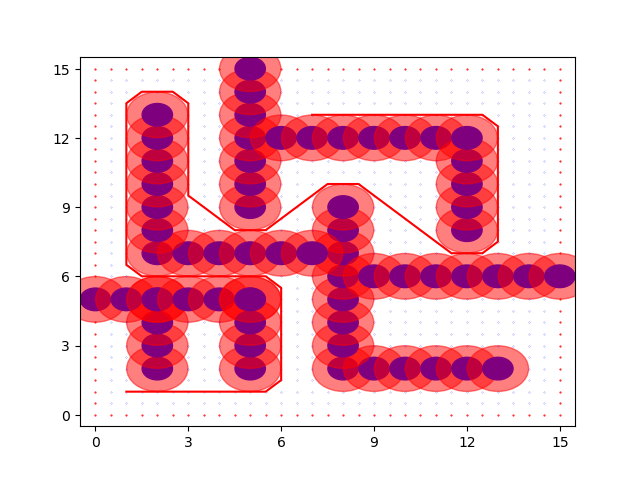
\includegraphics[width=\textwidth]{question1_dijkstras_path.png}
        \caption*{Dijkstra}
    \end {subfigure}
    \begin {subfigure} [b] {0.5\textwidth}
        \centering
        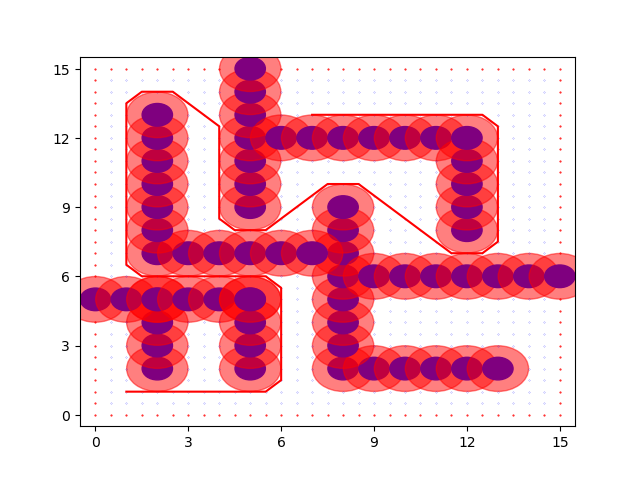
\includegraphics[width=\textwidth]{question1_astar_path.png}
        \caption*{A*}
    \end {subfigure}
    \begin {subfigure} [b] {0.5\textwidth}
        \centering
        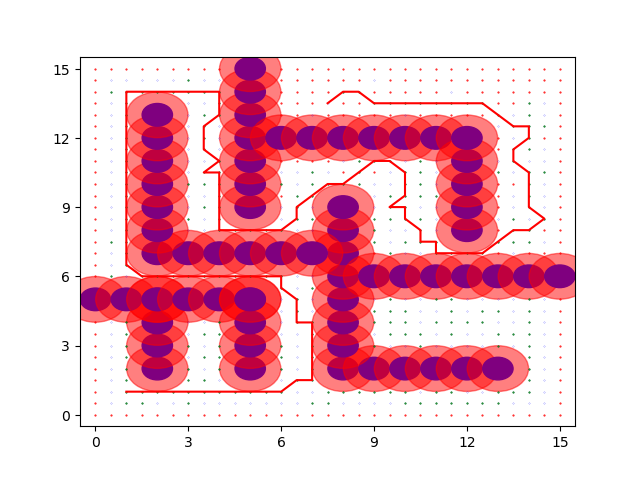
\includegraphics[width=\textwidth]{question1_rrt_path.png}
        \caption*{RRT}
    \end {subfigure}
\end{figure}

\bigskip
\begin{center}
    \begin{tabular}{ c c c }
        Agorithm & Path Length & Execution Time \\ 
        Dijsktras & 52.14 & 0.04 seconds \\
        A* & 52.14 & 0.017 seconds \\  
        RRT & 63.68 & 1.26 seconds \\

    \end{tabular}
\end{center}

Yes the results matched my expectations. Both Dijstra's and A* found the optimal path, with A* doing so a bit quicker because of the heuristic.
RRT also found a path, but as expected it is a bit "wobbly" due to it's random nature, and is slightly less optimal than the other two methods with a higher runtime.

\section*{Problem 2}
Using the obstacle list given below, run your A* and RRT within the ROS2 (and Gazebo)
environment. The turtlebot should follow the waypoints (just use the empty world for right now),
ensure that your turtlebot did not drive over any of the obstacle locations.
Show a plot with both the planned path and the actual turtlebot path.
Note: Use a robot size of 1.0 (or radius = 0.5) so you do not go through the obstacle list/walls

\bigskip
\noindent Start\_x = 1 \\
Start\_y = 1 \\
Goal\_x = 7 \\ 
Goal\_y = 13\\ \\
Obstacle\_x = [2, 2, 2, 2, 0, 1, 2, 3, 4, 5, 5, 5, 5, 5, 8, 9, 10, 11, 12, 13, 8, 8, 8, 8, 8, 8, 8, 2, 3, 4, 5, 6, 7,
9, 10, 11, 12, 13, 14, 15, 2, 2, 2, 2, 2, 2, 5, 5, 5, 5, 5, 5, 5, 6, 7, 8, 9, 10, 11, 12, 12, 12, 12, 12] \\ \\
Obstacle\_y = [2, 3, 4, 5, 5, 5, 5, 5, 5, 5, 2, 3, 4, 5, 2, 2, 2, 2, 2, 2, 3, 4, 5, 6, 7, 8, 9, 7, 7, 7, 7, 7, 7, 6, 6, 6,
6, 6, 6, 6, 8, 9, 10, 11, 12, 13, 9, 10, 11, 12, 13, 14, 15, 12, 12, 12, 12, 12, 12, 8, 9, 10, 11, 12] \\ \\
Max\_x = 15 \\
Max\_y = 15 \\ \\

\begin{figure}[H]
    \begin {subfigure} [b] {0.5\textwidth}
        \centering
        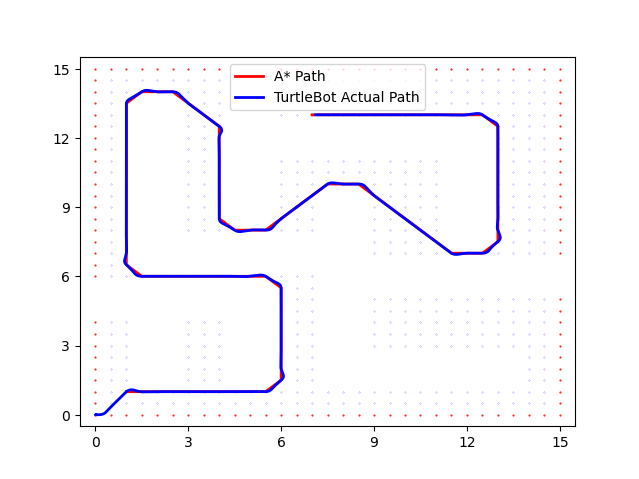
\includegraphics[width=\textwidth]{question2_astar.png}
        \caption*{A*}
    \end {subfigure}
    \begin {subfigure} [b] {0.5\textwidth}
        \centering
        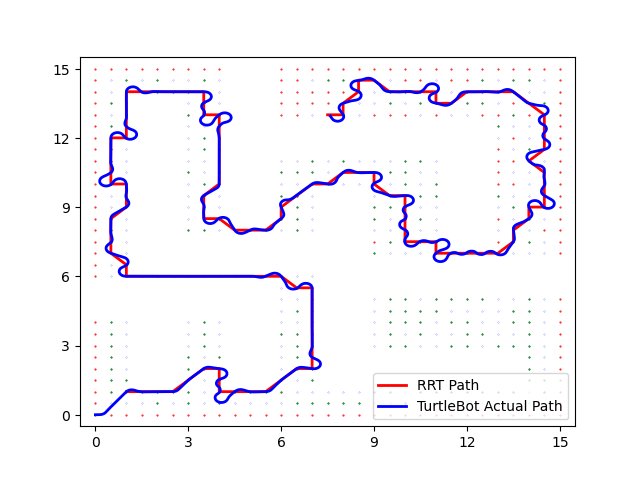
\includegraphics[width=\textwidth]{question2_rrt.png}
        \caption*{RRT}
    \end {subfigure}
\end{figure}

\noindent I made submodules from the code in previous homework. Then I ran the following code, swapping only line 22 when running RRT vs A*.

\begin{minted}[bgcolor=bg, linenos, frame=lines]{python}
def main(args=None):
    grid = Grid(0, 15, 0, 15, 0.5)

    obstacle_x = [2, 2, 2, 2, 0, 1, 2, 3, 4, 5, 5, 5, 5, 5, 8, 9, 
        10, 11, 12, 13, 8, 8, 8, 8, 8, 8, 8, 2, 3, 4, 5, 6, 7, 9,
        10, 11, 12, 13, 14, 15, 2, 2, 2, 2, 2, 2, 5, 5, 5, 5, 5,
        5, 5, 6, 7, 8, 9, 10, 11, 12, 12, 12, 12, 12]

    obstacle_y = [2, 3, 4, 5, 5, 5, 5, 5, 5, 5, 2, 3, 4, 5, 2, 2,
        2, 2, 2, 2, 3, 4, 5, 6, 7, 8, 9, 7, 7, 7, 7, 7, 7, 6, 6,
        6, 6, 6, 6, 6, 8, 9, 10, 11, 12, 13, 9, 10, 11, 12, 13,
        14, 15, 12, 12, 12, 12, 12, 12, 8, 9, 10, 11, 12]

    for x, y in zip(obstacle_x, obstacle_y):
        grid.add_obstacle(Obstacle(x, y, 0.49))
    
    grid.inflate(0.5)

    start = grid.nodes[(1,1)]
    end = grid.nodes[(7, 13)]

    x, y = grid.a_star(start,end)

    x.reverse()
    y.reverse()

    grid.draw(show_obstacles = False)

    plt.plot(x, y, color='red', linewidth=2, label='A* Path')
    
    rclpy.init(args=args)

    turtlebot_controller = TurtleBotController()

    turtlebot_controller.done = False
    
    for i in range(len(x)):
        turtlebot_controller.add_waypoint(x[i], y[i])
    
    while not turtlebot_controller.done:
        rclpy.spin_once(turtlebot_controller)
    

    plt.plot(turtlebot_controller.state_records['x'][0], 
        turtlebot_controller.state_records['y'][0], 
        color='blue', linewidth=2, label='TurtleBot Actual Path')
    
    plt.legend()
    plt.show()
    
    turtlebot_controller.destroy_node()
    rclpy.shutdown()


if __name__ == '__main__':
    main()

\end{minted}



\section*{Problem 3}

Write a script that solves the Traveling Salesman Problem (TSP) through brute force. Forth this
problem you simply need to compute the distance between the different waypoints/goal locations
(no path planning required). Show a plot that highlights the optimal path to go from the starting
point and visit the 4 waypoints with the minimum possible travelled distance.

\bigskip
\noindent Start = (0,0) \\
Goal 1 = (2,2)\\
Goal 2 = (5,3)\\
Goal 3 = (3,4)\\
Goal 4 = (6,4)\\

\bigskip
Note: You need to create a lookup table of the cost to go from any node to any other node (2
dimensional table). Use the distance as the cost for this problem. Then use a permutation package to
give you all possible permutations of the start connected with the 4 goals (4! Possibilities). You can
then go through these 4! possibilities and compute the total cost to travel. Find the minimum, and
that is your best path for the TSP.


\begin{figure}[h]
    \centering
    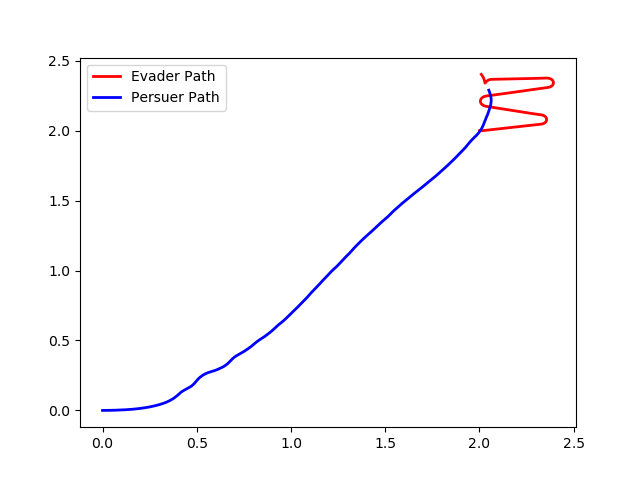
\includegraphics[width=0.5\textwidth]{question3.png}
    \caption*{TSP Solution}
    \label{fig:tsp}
\end{figure}

\noindent Path: \\
\indent Start (0, 0) \\
\indent Goal \#1 (2, 2) \\
\indent Goal \#3 (3, 4) \\
\indent Goal \#2 (5, 3) \\
\indent Goal \#4 (6, 4) \\ \\ 
Path Length: 8.714 \\

\begin{minted}[bgcolor=bg, linenos, frame=lines]{python}
from itertools import permutations
import math
import matplotlib.pyplot as plt
import multiprocessing

cities = [(2,2), (5,3), (3,4), (6,4)]

for city in cities:
    plt.scatter(city[0], city[1])


distances = {}

for city1 in cities:
    for city2 in cities:
        if city1 != city2:
            distances[(city1, city2)] = ((city1[0] - city2[0])**2 + (city1[1] - city2[1])**2)**0.5


minDistance = math.inf
minPath = None

for path in permutations(cities[1:]):
    path = (cities[0],) + path
    
    total_distance = 0
    for i in range(len(path)-1):
        total_distance += distances[(path[i], path[i+1])]
    
    if total_distance < minDistance:
        minDistance = total_distance
        minPath = path


print(f"Shortest path is {minPath} with a distance of {minDistance}")

plt.annotate("Start", minPath[0])

for i in range(1, len(minPath)):
    current_city = minPath[i]
    previous_city = minPath[i-1]

    plt.annotate(f"Goal {cities.index(current_city) + 1}", current_city)
    plt.plot([current_city[0], previous_city[0]], [current_city[1], previous_city[1]], color='red')

plt.show()
\end{minted}
\end{document}